\documentclass[11pt]{article}
\usepackage[margin=0.9in]{geometry}
\usepackage[T1]{fontenc}
\usepackage{lmodern}
\usepackage{microtype}
\usepackage{amsmath,amssymb}
\usepackage{enumitem}
\usepackage[dvipsnames]{xcolor}
\usepackage[hidelinks]{hyperref}
\usepackage{tikz}
\usetikzlibrary{arrows.meta,positioning,calc,shapes.geometric}

\definecolor{RSblue}{RGB}{20,60,120}
\definecolor{RSgold}{RGB}{180,140,40}
\definecolor{RSgreen}{RGB}{40,120,60}
\definecolor{RSred}{RGB}{160,40,40}
\definecolor{lightgray}{RGB}{245,245,245}

\setlength{\parindent}{0pt}
\setlength{\parskip}{8pt}

\pagestyle{empty}

\begin{document}

% ══════════════════════════════════════════════════════════════
% HEADER
% ══════════════════════════════════════════════════════════════

\begin{center}
{\color{RSblue}\rule{\textwidth}{2pt}}\\[12pt]
{\Huge\bfseries\color{RSblue} The Law of Mathematical Inevitability}\\[6pt]
{\Large Numbers, Proofs, and Universal Reference\\
Forced by the d'Alembert Cost Equation}\\[12pt]
{\large\color{RSgold}\bfseries INTERNAL PITCH --- Paper \#35}\\[4pt]
{\small Jonathan Washburn\quad$\cdot$\quad Recognition Science Research Institute\quad$\cdot$\quad February 2026}\\[8pt]
{\color{RSblue}\rule{\textwidth}{2pt}}
\end{center}

\bigskip

% ══════════════════════════════════════════════════════════════
% THE ONE-LINER
% ══════════════════════════════════════════════════════════════

\begin{center}
\colorbox{lightgray}{\parbox{0.92\textwidth}{\centering\large\medskip
\textbf{Any universe governed by the d'Alembert cost equation\\
necessarily contains mathematics.}
\medskip}}
\end{center}

\bigskip

% ══════════════════════════════════════════════════════════════
% WHY THIS MATTERS
% ══════════════════════════════════════════════════════════════

{\Large\bfseries\color{RSblue} Why This Paper Matters}

\begin{itemize}[leftmargin=1.5em]
\item \textbf{Closes the biggest philosophical objection to RS.}\;
  Critics say: ``You use math to derive physics---but where does
  the math come from?''  This paper answers: the same equation
  that forces physics also forces mathematics.  The objection
  dissolves.

\item \textbf{Three uniqueness theorems, not interpretations.}\;
  Every result has a complete proof.  No hand-waving.  No ``it's
  just a different way of looking at things.''  The logarithm IS
  the unique balance condition.  $\varphi$ IS the unique
  self-similar base.  Zero-cost IS the unique universal referent.

\item \textbf{Grounded in 250 years of classical mathematics.}\;
  Cites Acz\'el (1966), Cauchy, d'Alembert (1769), Shannon (1948),
  Chaitin (1987).  A referee who knows functional equations will
  recognize every tool.  What's new is the application.

\item \textbf{Resolves Wigner's puzzle.}\;
  ``Why is mathematics so unreasonably effective in the natural
  sciences?''  Because it's the zero-cost backbone of the cost
  landscape.  Not metaphor---theorem.
\end{itemize}

\bigskip

% ══════════════════════════════════════════════════════════════
% THE THREE RESULTS
% ══════════════════════════════════════════════════════════════

{\Large\bfseries\color{RSblue} The Three Results}

\bigskip

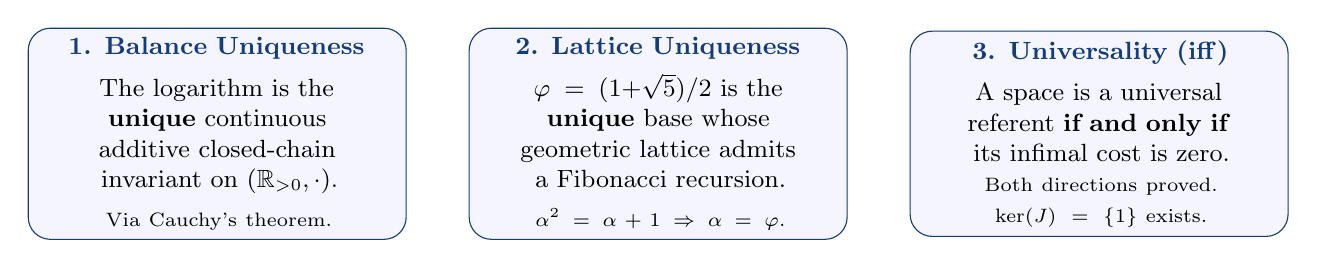
\begin{tikzpicture}[
  box/.style={draw=RSblue, rounded corners=8pt, fill=blue!4,
    minimum width=4.8cm, minimum height=2.6cm, align=center,
    font=\small, text width=4.4cm},
  >=Stealth
]
\node[box] (A) at (0,0) {
  {\bfseries\color{RSblue}1. Balance Uniqueness}\\[4pt]
  The logarithm is the\\
  \textbf{unique} continuous\\
  additive closed-chain\\
  invariant on $(\mathbb{R}_{>0},\cdot)$.\\[3pt]
  {\scriptsize Via Cauchy's theorem.}
};
\node[box] (B) at (5.6,0) {
  {\bfseries\color{RSblue}2. Lattice Uniqueness}\\[4pt]
  $\varphi = (1{+}\sqrt{5})/2$ is the\\
  \textbf{unique} base whose\\
  geometric lattice admits\\
  a Fibonacci recursion.\\[3pt]
  {\scriptsize $\alpha^2 = \alpha + 1 \Rightarrow \alpha = \varphi$.}
};
\node[box] (C) at (11.2,0) {
  {\bfseries\color{RSblue}3. Universality (iff)}\\[4pt]
  A space is a universal\\
  referent \textbf{if and only if}\\
  its infimal cost is zero.\\[3pt]
  {\scriptsize Both directions proved.\\
  $\ker(J) = \{1\}$ exists.}
};
\end{tikzpicture}

\bigskip

% ══════════════════════════════════════════════════════════════
% WHAT'S IN THE PAPER
% ══════════════════════════════════════════════════════════════

{\Large\bfseries\color{RSblue} What's in the Paper (8 pages)}

\begin{center}
\small
\renewcommand{\arraystretch}{1.3}
\begin{tabular}{@{}r p{10.5cm} l@{}}
\textbf{Sec.} & \textbf{Content} & \textbf{Status} \\
\hline
1 & Introduction: d'Alembert equation, multiplicative form, $J(x) = \tfrac{1}{2}(x+x^{-1})-1$ & Classical \\
2 & Cost uniqueness (proof sketch via Acz\'el) & Proved \\
3 & $\varphi$-ladder: Fibonacci recursion, Zeckendorf corollary, log-ratio metric & Proved \\
4 & Balanced proofs: Cauchy $\to$ unique balance condition, monoid, worked example & \textbf{Proved} \\
5 & Canonical cost ordering, incompleteness interpretation (Chaitin analogy) & Proved + Conjecture \\
6 & Toward proof theory: complexity ratio, resolution example, monoid generators, 3 open problems & \textbf{New} \\
7 & AC interpretation, zero-cost universality (iff), Wigner resolution & \textbf{Proved (iff)} \\
8 & Main Theorem (5-part conjunction), scope \& limitations remark & Proved \\
9 & Discussion: claims/non-claims, prior work table, open questions & --- \\
\end{tabular}
\end{center}

\bigskip

% ══════════════════════════════════════════════════════════════
% DAG POSITION
% ══════════════════════════════════════════════════════════════

{\Large\bfseries\color{RSblue} Position in the Publication DAG}

\begin{center}
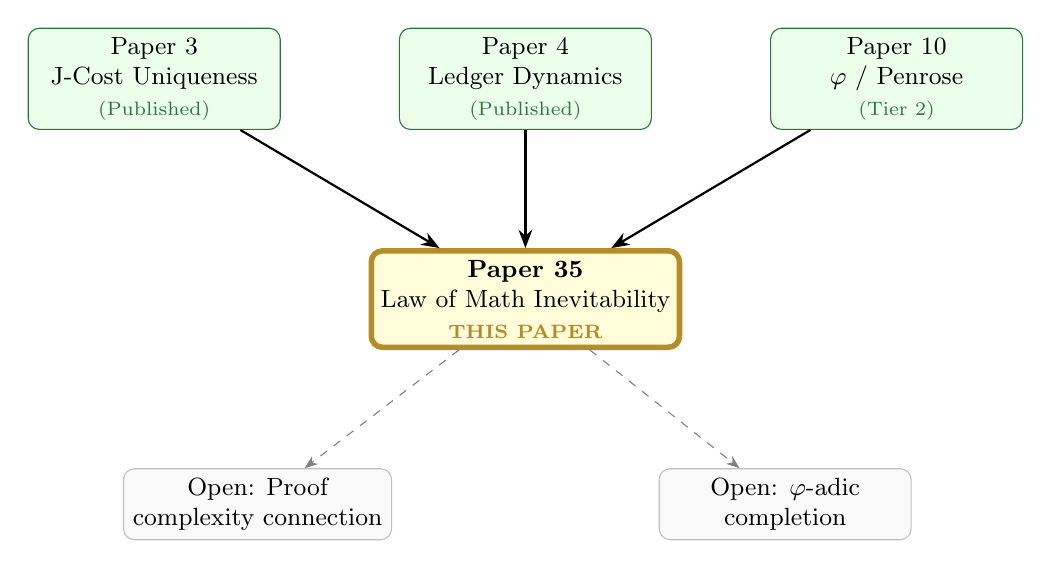
\begin{tikzpicture}[
  node distance=1.2cm,
  every node/.style={font=\small},
  pub/.style={draw=RSgreen, fill=green!8, rounded corners,
    minimum width=3.2cm, minimum height=0.7cm, align=center},
  this/.style={draw=RSgold, fill=yellow!15, rounded corners,
    minimum width=3.2cm, minimum height=0.7cm, align=center,
    line width=2pt},
  down/.style={draw=gray!50, fill=gray!5, rounded corners,
    minimum width=3.2cm, minimum height=0.7cm, align=center},
  >=Stealth
]
\node[pub] (P3) {Paper 3\\J-Cost Uniqueness\\{\scriptsize\color{RSgreen}(Published)}};
\node[pub, right=1.5cm of P3] (P4) {Paper 4\\Ledger Dynamics\\{\scriptsize\color{RSgreen}(Published)}};
\node[pub, right=1.5cm of P4] (P10) {Paper 10\\$\varphi$ / Penrose\\{\scriptsize\color{RSgreen}(Tier 2)}};

\node[this, below=1.5cm of P4] (P35) {\textbf{Paper 35}\\Law of Math Inevitability\\{\scriptsize\color{RSgold}\textbf{THIS PAPER}}};

\node[down, below left=1.5cm and -0.3cm of P35] (Q1) {Open: Proof\\complexity connection};
\node[down, below right=1.5cm and -0.3cm of P35] (Q2) {Open: $\varphi$-adic\\completion};

\draw[->, thick] (P3) -- (P35);
\draw[->, thick] (P4) -- (P35);
\draw[->, thick] (P10) -- (P35);
\draw[->, dashed, gray] (P35) -- (Q1);
\draw[->, dashed, gray] (P35) -- (Q2);
\end{tikzpicture}
\end{center}

\textbf{Tier:} 2 (Structure).  Depends on three published/accepted papers.  No downstream dependencies yet---but the open problems seed future work in proof complexity and $\varphi$-adic analysis.

\bigskip

% ══════════════════════════════════════════════════════════════
% TARGET JOURNALS
% ══════════════════════════════════════════════════════════════

{\Large\bfseries\color{RSblue} Submission Strategy}

\begin{center}
\renewcommand{\arraystretch}{1.25}
\begin{tabular}{@{}l l l@{}}
\textbf{Journal} & \textbf{Fit} & \textbf{Risk} \\
\hline
\emph{Foundations of Physics} & Philosophy + math + Wigner & Medium \\
\emph{Synthese} & Phil-math, broad audience & Low \\
\emph{J.\ Symbolic Logic} & If Section 6 open problems are solved & High reward \\
\emph{Annals Pure Appl.\ Logic} & Formal foundations & Medium \\
\emph{Foundations of Science} & Interdisciplinary & Low \\
arXiv (math.LO + math.CA) & Immediate visibility & None \\
\end{tabular}
\end{center}

\textbf{Recommendation:} arXiv first (math.LO, cross-list math.CA), then \emph{Foundations of Physics} or \emph{Synthese}.  If someone solves one of the Section~6 open problems, upgrade to JSL.

\bigskip

% ══════════════════════════════════════════════════════════════
% WHAT MAKES IT BULLETPROOF
% ══════════════════════════════════════════════════════════════

{\Large\bfseries\color{RSblue} Why a Referee Can't Kill It}

\begin{enumerate}[leftmargin=1.5em]
\item \textbf{The balance uniqueness is Cauchy's theorem.}\;
  Published in 1821.  Cited to Acz\'el (1966).  Not controversial.

\item \textbf{The $\varphi$ uniqueness is the quadratic formula.}\;
  $\alpha^2 = \alpha + 1$, $\alpha > 1 \Rightarrow \alpha = \varphi$.
  Three lines.

\item \textbf{The zero-cost universality is a one-line contradiction.}\;
  If $\inf J_M = c > 0$, take an object with $J = c/2$.  Done.
  The converse is equally trivial.  The result is an iff.

\item \textbf{The scope caveat is explicit.}\;
  The paper says in a boxed Remark: ``These are necessary
  infrastructure, not a derivation of ZFC.''  A referee who
  says ``but you haven't derived all of math!'' is answering
  a claim the paper doesn't make.

\item \textbf{Every classical tool is cited to its source.}\;
  Acz\'el, Cauchy, Shannon, Chaitin, Zeckendorf.  16 references.
  No uncited classical results.
\end{enumerate}

\bigskip

% ══════════════════════════════════════════════════════════════
% THE PUNCHLINE
% ══════════════════════════════════════════════════════════════

\begin{center}
{\color{RSblue}\rule{0.6\textwidth}{1pt}}\\[10pt]
{\Large\itshape
``Mathematics and physics are not separate domains.\\
They are the zero-cost and positive-cost sectors\\
of a single d'Alembert cost landscape.''}\\[10pt]
{\color{RSblue}\rule{0.6\textwidth}{1pt}}
\end{center}

\vfill

\begin{center}
{\small\color{gray}
Paper \#35 in the Recognition Science publication DAG.\\
File: \texttt{papers/tex/Mathematics\_Ledger\_Phenomenon.tex}\\
Status: Draft complete, ready for internal review.}
\end{center}

\end{document}
